%----------------------------------------------------------------------------------------
%	PACKAGES AND OTHER DOCUMENT CONFIGURATIONS
%----------------------------------------------------------------------------------------

\documentclass[10pt]{report}

\usepackage[a4paper,pdftex]{geometry}	% Use A4 paper margins
\usepackage[dutch]{babel}
%\usepackage[T1]{fontenc}           % For font
%\usepackage[garamond]{mathdesign}  % For font
\usepackage{amsmath}
\usepackage{amsfonts}
\usepackage{amssymb}
\usepackage{amsthm}
\usepackage{subfiles}
\usepackage{graphicx}
\usepackage{algorithm} % For algorithms
\usepackage{algorithmic} % For algorithms
\usepackage{float}
\usepackage{tikz}
\usepackage{rotating} % for sideways figures
\usepackage{xcolor} % Required for specifying custom colors
\usepackage{fix-cm} % Allows increasing the font size of specific fonts beyond LaTeX default specifications

\AtBeginDocument{
  \renewcommand\chaptername{Vraag}
}

\begin{document}
\begin{titlepage}


\thispagestyle{empty} % Remove page numbering on this page


\newcommand{\HRule}{\rule{\linewidth}{0.5mm}} % Defines a new command for the horizontal lines, change thickness here

\center % Center everything on the page
 
%----------------------------------------------------------------------------------------
%	HEADING SECTIONS
%----------------------------------------------------------------------------------------

\textsc{\LARGE KU Leuven}\\[1.5cm] % Name of your university/college
\textsc{\Large Artifici\"ele Intelligentie}\\[0.5cm] % Major heading such as course name
%\textsc{\large Minor Heading}\\[0.5cm] % Minor heading such as course title

%----------------------------------------------------------------------------------------
%	TITLE SECTION
%----------------------------------------------------------------------------------------

\HRule \\[0.4cm]
{ \Huge \bfseries Alternatief Examen}\\
\HRule \\[2cm]
 
%----------------------------------------------------------------------------------------
%	AUTHOR SECTION
%----------------------------------------------------------------------------------------

\begin{minipage}{0.4\textwidth}
\begin{flushleft} \large
\emph{Auteur:}\\
Tom Sydney \textsc{Kerckhove} % Your name
\end{flushleft}
\end{minipage}
~
\begin{minipage}{0.4\textwidth}
\begin{flushright} \large
\emph{Professor:} \\
Danny \textsc{De Schreye} % Supervisor's Name
\end{flushright}
\end{minipage}\\[1cm]

\begin{minipage}{0.4\textwidth}
\begin{flushleft} \large
\emph{R-nummer:}\\
r0372924 % Your name
\end{flushleft}
\end{minipage}
~
\begin{minipage}{0.4\textwidth}
\begin{flushright} \large
\emph{Righting:} \\
Bachelor of science in de Informatica, 2e fase % Supervisor's Name
\end{flushright}
\end{minipage}

\begin{center}
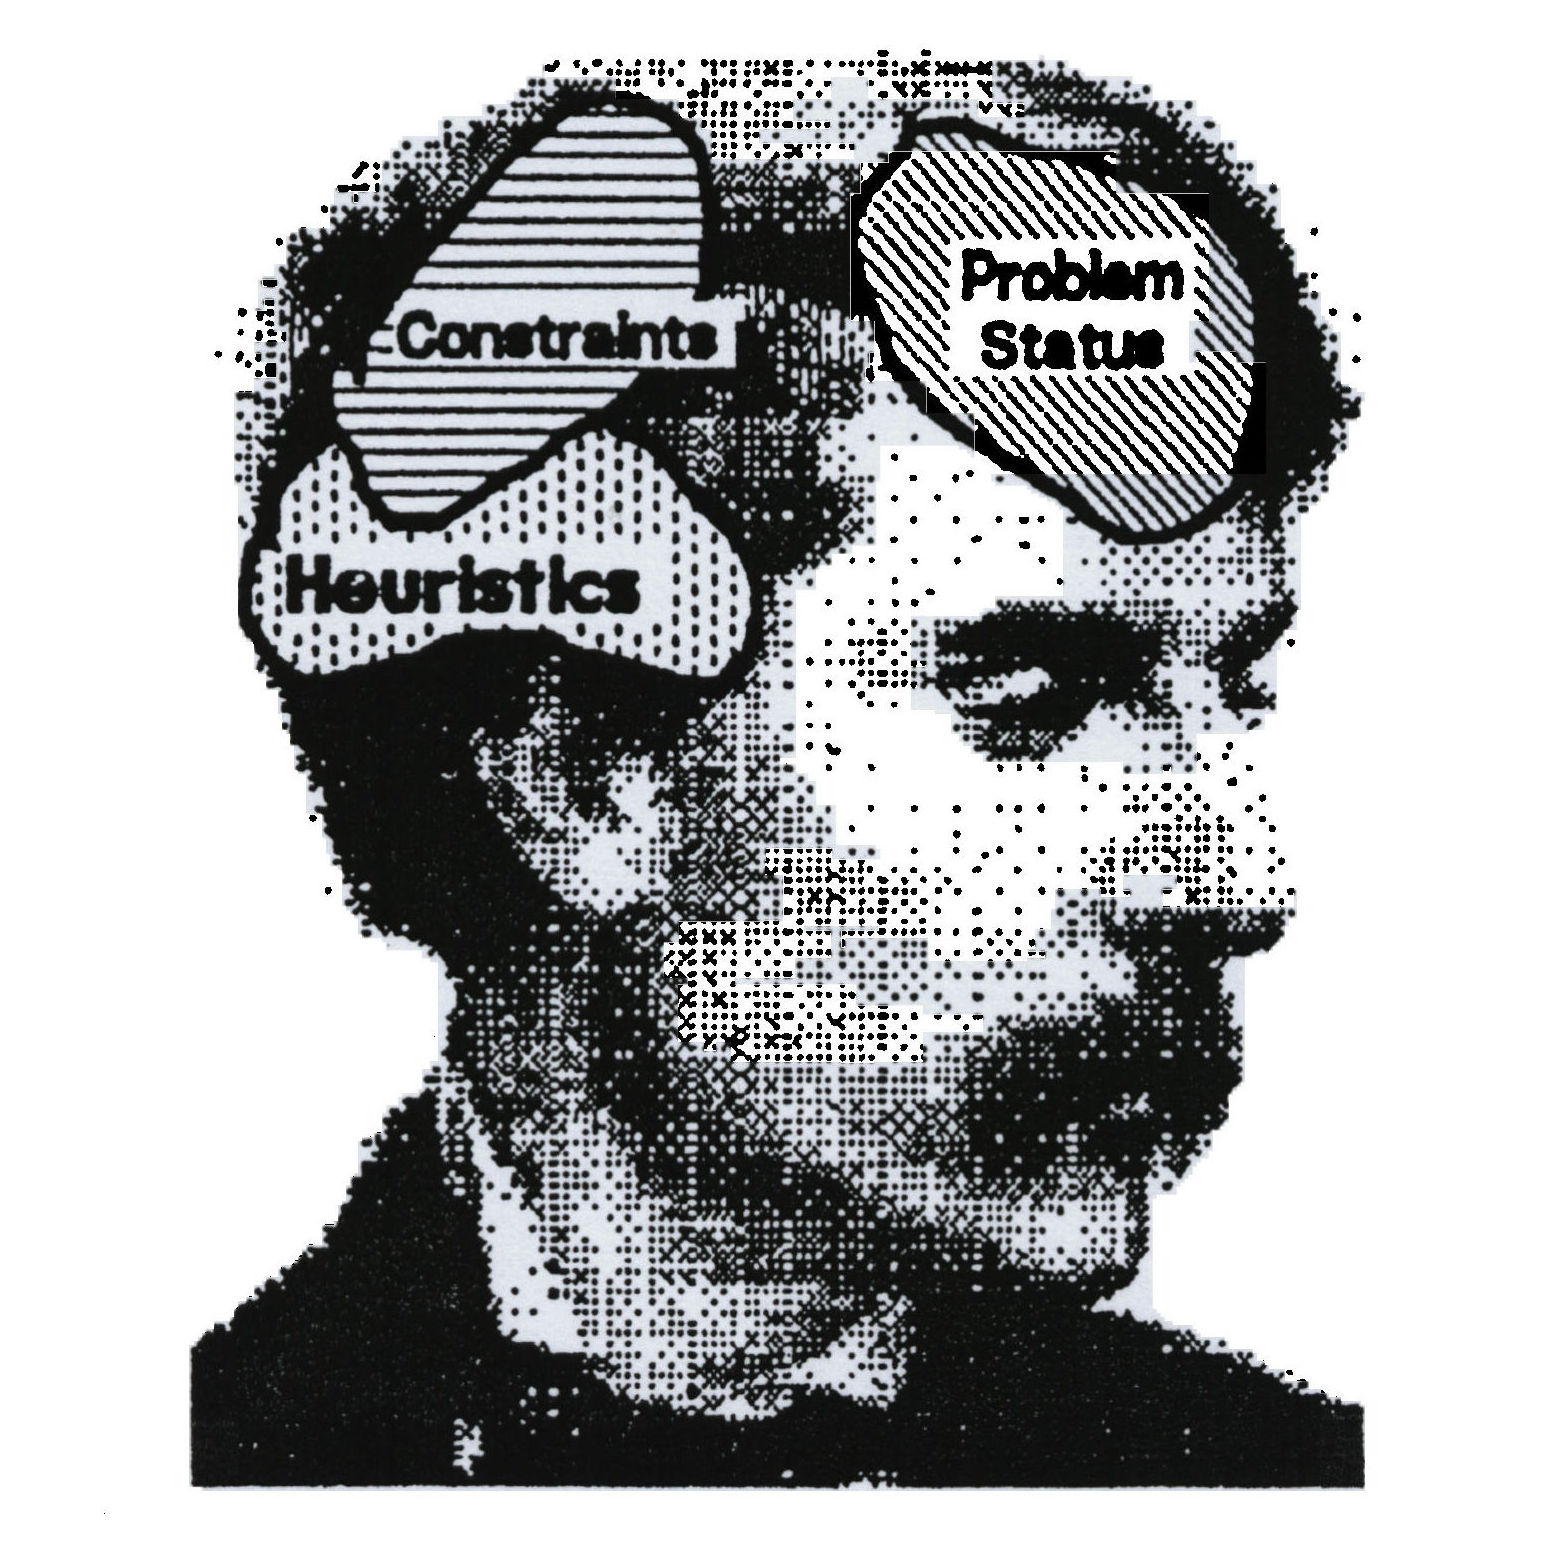
\includegraphics[scale=0.15]{resources/pictures/ai.jpg}
\end{center}

%----------------------------------------------------------------------------------------
%	DATE SECTION
%----------------------------------------------------------------------------------------

{\large 13 januari 2014}\\[3cm]

%----------------------------------------------------------------------------------------
%	LOGO SECTION
%----------------------------------------------------------------------------------------

%\includegraphics{Logo}\\[1cm] % Include a department/university logo - this will require the graphicx package
 
%----------------------------------------------------------------------------------------

\vfill % Fill the rest of the page with whitespace

\end{titlepage}
\newpage

\subfile{ai_inleiding}
\tableofcontents
\subfile{ai_vraag_1}
\subfile{ai_vraag_2}
\subfile{ai_vraag_3}
\subfile{ai_vraag_4}
\subfile{ai_vraag_5}
\subfile{ai_reflectie}

\subfile{ai_appendix}

\end{document}